\documentclass[sigconf,10pt,nonacm]{acmart}

%% ---------------------------------------------------------------- bibliography
\begin{filecontents*}[overwrite]{refs.bib}
@misc{brief,
  author       = {{National University of Singapore}},
  title        = {{CS4224/CS5424} Project},
  year         = {2026},
  howpublished = {\url{https://canvas.nus.edu.sg/courses/96671/pages/project}},
}
@book{ozsu2020,
  author    = {M. Tamer {\"O}zsu and Patrick Valduriez},
  title     = {Principles of Distributed Database Systems},
  edition   = {Fourth},
  publisher = {Springer},
  year      = {2020},
  doi       = {10.1007/978-3-030-26253-2},
}
@book{rahimi2010,
  author    = {Saeed K. Rahimi and Frank S. Haug},
  title     = {Distributed Database Management Systems: A Practical Approach},
  publisher = {Wiley-IEEE Computer Society Press},
  year      = {2010},
}
@article{liu2024survey,
  author  = {Peng-Ju Liu and Cui-Ping Li and Hong Chen},
  title   = {Enhancing Storage Efficiency and Performance: A Survey of Data Partitioning Techniques},
  journal = {Journal of Computer Science and Technology},
  volume  = {39},
  number  = {2},
  pages   = {346--368},
  year    = {2024},
  doi     = {10.1007/s11390-024-3538-1},
}
@article{navathe1984,
  author  = {Shamkant Navathe and Stefano Ceri and Gio Wiederhold and Jinglie Dou},
  title   = {Vertical Partitioning Algorithms for Database Design},
  journal = {ACM Transactions on Database Systems},
  volume  = {9},
  number  = {4},
  pages   = {680--710},
  year    = {1984},
}
@article{mccormick1972,
  author  = {William T. McCormick and Paul J. Schweitzer and Thomas W. White},
  title   = {Problem Decomposition and Data Reorganization by a Clustering Technique},
  journal = {Operations Research},
  volume  = {20},
  number  = {5},
  pages   = {993--1009},
  year    = {1972},
}
@inproceedings{hankins2003,
  author    = {Richard A. Hankins and Jignesh M. Patel},
  title     = {Data Morphing: An Adaptive, Cache-Conscious Storage Technique},
  booktitle = {Proceedings of the 29th International Conference on Very Large Data Bases (VLDB)},
  pages     = {417--428},
  year      = {2003},
}
@inproceedings{papadomanolakis2004,
  author    = {Stratos Papadomanolakis and Anastassia Ailamaki},
  title     = {{AutoPart}: Automating Schema Design for Large Scientific Databases Using Data Partitioning},
  booktitle = {Proceedings of the 16th International Conference on Scientific and Statistical Database Management (SSDBM)},
  pages     = {383--392},
  year      = {2004},
}
@article{jindal2013,
  author  = {Alekh Jindal and Endre Palatinus and Vladimir Pavlov and Jens Dittrich},
  title   = {A Comparison of Knives for Bread Slicing},
  journal = {Proceedings of the VLDB Endowment},
  volume  = {6},
  number  = {6},
  pages   = {361--372},
  year    = {2013},
}
@manual{pgisolation,
  author       = {{PostgreSQL Global Development Group}},
  title        = {{PostgreSQL} 18 Documentation, Section 13.2: Transaction Isolation},
  year         = {2025},
  howpublished = {\url{https://www.postgresql.org/docs/18/transaction-iso.html}},
}
@manual{pgadvisory,
  author       = {{PostgreSQL Global Development Group}},
  title        = {{PostgreSQL} 18 Documentation, Section 13.3.5: Advisory Locks},
  year         = {2025},
  howpublished = {\url{https://www.postgresql.org/docs/18/explicit-locking.html}},
}
@manual{pgindexonly,
  author       = {{PostgreSQL Global Development Group}},
  title        = {{PostgreSQL} 18 Documentation, Section 11.9: Index-Only Scans and Covering Indexes},
  year         = {2025},
  howpublished = {\url{https://www.postgresql.org/docs/18/indexes-index-only-scans.html}},
}
@manual{pgvisibilitymap,
  author       = {{PostgreSQL Global Development Group}},
  title        = {{PostgreSQL} 18 Documentation, Section 66.4: Visibility Map},
  year         = {2025},
  howpublished = {\url{https://www.postgresql.org/docs/18/storage-vm.html}},
}
@manual{pgssi,
  author       = {{PostgreSQL Global Development Group}},
  title        = {{PostgreSQL} 18 Source, {README-SSI}},
  year         = {2025},
  howpublished = {\url{https://github.com/postgres/postgres/blob/REL_18_STABLE/src/backend/storage/lmgr/README-SSI}},
}
@manual{citustx,
  author       = {{Citus Data}},
  title        = {Citus 14.1.0 Source: \texttt{remote\_transaction.c} and \texttt{transaction\_management.c}},
  year         = {2025},
  howpublished = {\url{https://github.com/citusdata/citus/tree/v14.1.0/src/backend/distributed/transaction}},
}
\end{filecontents*}

%% ---------------------------------------------------------------- packages
\settopmatter{printacmref=false, printccs=false, printfolios=true}
\renewcommand\footnotetextcopyrightpermission[1]{}
\pagestyle{plain}

\usepackage{siunitx}
\sisetup{group-separator={,}, group-minimum-digits=4}
\usepackage{pgfplots}
\pgfplotsset{compat=1.18}
\usetikzlibrary{arrows.meta, positioning, fit}
\usepackage[capitalise, noabbrev]{cleveref}
\usepackage{array}
\newcolumntype{L}[1]{>{\raggedright\arraybackslash}p{#1}}

\newcommand{\expt}[1]{\texttt{expt\textunderscore #1}}
\let\underscorewithoutbreak\_
\renewcommand{\_}{\underscorewithoutbreak\allowbreak}
\emergencystretch=4em
\newcommand{\ab}[1]{\texttt{a#1}/\texttt{b#1}}

%% ---------------------------------------------------------------- front matter
\title{Optimizing Transaction Processing on Citus}
\subtitle{CS4224/CS5424 Project, Team 08}

\author{Christopher Terence Ng}
\affiliation{\institution{National University of Singapore}\country{Singapore}}
\author{Don Tay Xi Cheng}
\affiliation{\institution{National University of Singapore}\country{Singapore}}
\author{Timothy Josef Ho}
\affiliation{\institution{National University of Singapore}\country{Singapore}}
\author{Yong Kotaro}
\affiliation{\institution{National University of Singapore}\country{Singapore}}

\renewcommand{\shortauthors}{Team 08}

\begin{abstract}
Citus scales PostgreSQL by spreading tables across worker nodes, but it enforces
serializable isolation only within each worker. We optimize a multi-tenant
order-processing benchmark on a five-node Citus~14.1 cluster for two transaction mixes,
A and B, while requiring the final designs to be serializable across the whole cluster. Our baseline
achieves this with two-phase locking on the coordinator and reaches 1.3 transactions
per second (TPS) on workload A and 3.2~TPS on workload B at 64 clients. Query rewrites,
partitioning every table by merchant, and a covering index raise throughput to 625~TPS
on workload A. The same steps, plus a vertical split of the orders table, raise
workload B to 446~TPS. None of our serializable designs had a serialization failure or
an aborted client.

Profiling explains most of this gain. Once the other transactions were fast, the
global sales report (T6) took 94--96\% of all transaction time, because every
execution scanned all five million orders. An index that answers T6 without reading
the table raised throughput at 64 clients by $8.3\times$ on workload A and $10.9\times$
on workload B. We also evaluated three classical vertical partitioning algorithms.
While T6 scanned the table, two of their designs made no measurable difference and the
third was 28\% slower. After the index was added, the split proposed by Navathe et al.\
made T6 18--20\% faster on both workloads, but it also gives every new order a second
insert. On workload A, where most transactions place orders, throughput stayed within
5\%. On workload B, it rose by 7\% at 32 and 64 clients.
\end{abstract}

\begin{document}
\maketitle

\noindent\textbf{AI tools used.} GPT-6.1 Sol (OpenAI), to outline the report. Claude
Code with Claude Opus 5.5, Claude Sonnet 5.5 and Claude Fable 5.1 (Anthropic), to
implement and test the vertical partitioning algorithms, the experiment tooling and the
experiments built on them, to analyse benchmark results, and to draft and edit the text
of this report. The interactions are submitted in \texttt{08\_ai\_tool.zip}.

%% ================================================================ Section 1
\section{Team Member Contributions}
\label{sec:contributions}

\textbf{Christopher Terence Ng} built the infrastructure for testing and benchmarking:
a Docker replica of the SoC cluster's Slurm setup (the \emph{Local Cluster}),
continuous integration that tests every experiment of a pull request on that replica
(the \emph{GitHub Cluster}), and scripts that run benchmarks on the SoC cluster and
link each result to the git commit that produced it. He implemented three classical
vertical partitioning algorithms (Navathe et al.'s affinity-based algorithm, the
Hill-Climb algorithm of Data Morphing, and AutoPart) and benchmarked their designs
(\expt{a103}, \expt{a113}, \expt{a123}). He profiled the combined design, found that
T6 dominated it, added T6's covering index (\expt{a205}, \expt{b205}), and tested two of
the vertical partitions on top of that index (\expt{a206}, \expt{a207}, \expt{b206},
\expt{b207}).

\textbf{Don Tay Xi Cheng} designed the \emph{serializable baseline}, our reference
design for measuring optimization gains (\expt{a99},
\expt{b99}), including the coordinator locks, snapshot initialization under an exclusive lock for T6 and its
correctness argument. He also wrote the query-rewrite chains for both workloads
(\expt{a101}--\expt{a131}, \expt{b101}--\expt{b131}).

\textbf{Timothy Josef Ho} added indexes (\expt{a104}, \expt{b104}), partitioned all
tables by merchant (\expt{a114}, \expt{b114}), and combined these ideas with Don's
query rewrites and an order-routing table into the combined design (\expt{a204},
\expt{b204}).

\textbf{Yong Kotaro} implemented and analysed three denormalization designs: an order
history keyed by customer (\expt{a102}, \expt{b102}), a merged product and inventory
table (\expt{a112}, \expt{b112}), and a split of product data into hot and cold tables. (\expt{a122}, \expt{b122}).

\clearpage

%% ================================================================ Section 2
\section{Task 1: Baseline Design for Workload A}
\label{sec:task1}

\subsection{Benchmark Method}
\label{sec:method}

\paragraph{Setup.} All experiments run the supplied \texttt{run.sh} on five nodes of the
SoC compute cluster. The first node is the Citus coordinator and also runs pgbench; the
other four are workers. Unless we state otherwise, each node receives four CPUs, as in
the supplied script, and pgbench uses four threads. The data is generated at
\texttt{SCALE=1}: 1,000 merchants, 1 million customers, 500,000 products, 5 million
orders and 15 million order items~\cite{brief}. For each of 1, 4, 8, 16, 32 and 64
concurrent clients, a run reloads the data, restarts the servers, warms up for 60\,s
and then measures for 600\,s. pgbench tries each transaction up to three times, and it
retries only after a serialization failure or a deadlock. Throughput, in transactions
per second (TPS), is the number of successful transactions divided by 600\,s, as
computed by the supplied scripts. Latency percentiles come from the same transaction
logs.

\paragraph{Threshold.} We ran each configuration once. We use 10\% as a descriptive
threshold for highlighting throughput differences. Because each configuration has only
one run, this threshold neither estimates noise nor establishes statistical
significance.

\paragraph{Tooling.} A benchmark run takes about 100 minutes on the shared cluster, so
we checked every change before submitting it. The \emph{Local Cluster} reproduces the
cluster's Slurm and Citus setup in Docker containers, where an experiment runs at a
reduced scale in a few minutes on a developer's machine. The \emph{GitHub Cluster} runs
the same check, in GitHub Actions, for every experiment in a pull request. Experiments
that pass are benchmarked on the SoC cluster by scripts that submit the job, wait for
it, copy the results back and record the git commit that produced them. All numbers in
this report come from the SoC cluster.

\paragraph{Experiments.} \Cref{fig:lineage} shows how the experiments build on one
another. We name an experiment \texttt{a}$N$ or \texttt{b}$N$ for workload A or B. The
two experiments of one number are counterparts in the two workloads, which differ only
in the order of the query rewrites (see the caption). Four experiments exist for
workload A only: \expt{a100}, \expt{a103}, \expt{a113} and \expt{a123}.

\begin{figure*}[t]
\centering
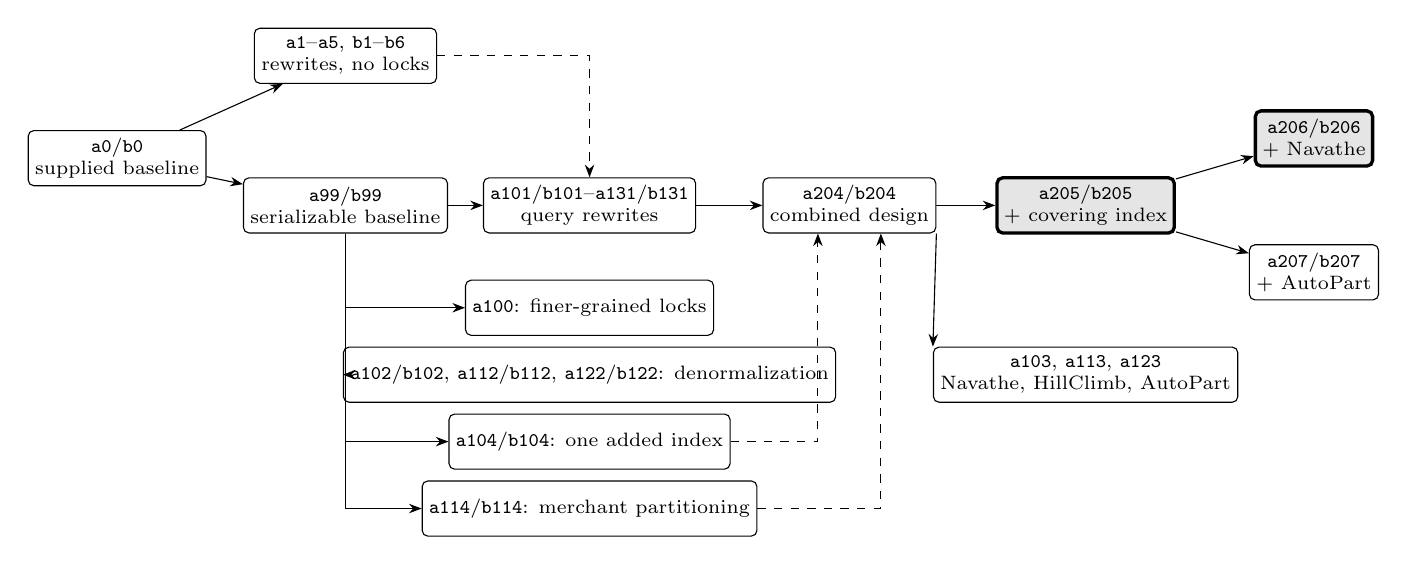
\begin{tikzpicture}[
    experiment/.style={draw, rounded corners=2pt, font=\scriptsize, align=center, inner sep=2.5pt, minimum height=7mm},
    final/.style={experiment, very thick, fill=black!10},
    builds/.style={-{Stealth[length=1.6mm]}},
    informs/.style={-{Stealth[length=1.6mm]}, dashed},
  ]
  \node[experiment] (a0)     at (0, 0)      {\ab{0}\\supplied baseline};
  \node[experiment] (a1)     at (2.9, 1.3)  {\texttt{a1}--\texttt{a5}, \texttt{b1}--\texttt{b6}\\rewrites, no locks};
  \node[experiment] (a99)    at (2.9, -0.6) {\ab{99}\\serializable baseline};
  \node[experiment] (chain)  at (6.0, -0.6) {\ab{101}--\ab{131}\\query rewrites};
  \node[experiment] (a204)   at (9.3, -0.6) {\ab{204}\\combined design};
  \node[final]      (a205)   at (12.3, -0.6){\ab{205}\\+ covering index};
  \node[final]      (a206)   at (15.2, 0.25){\ab{206}\\+ Navathe};
  \node[experiment] (a207)   at (15.2, -1.45){\ab{207}\\+ AutoPart};
  \node[experiment] (a100)   at (6.0, -1.9) {\texttt{a100}: finer-grained locks};
  \node[experiment] (denorm) at (6.0, -2.75){\ab{102}, \ab{112}, \ab{122}: denormalization};
  \node[experiment] (a104)   at (6.0, -3.6) {\ab{104}: one added index};
  \node[experiment] (a114)   at (6.0, -4.45){\ab{114}: merchant partitioning};
  \node[experiment] (vp)     at (12.3, -2.75){\texttt{a103}, \texttt{a113}, \texttt{a123}\\Navathe, HillClimb, AutoPart};

  \draw[builds] (a0) -- (a1);
  \draw[builds] (a0) -- (a99);
  \draw[builds] (a99) -- (chain);
  \draw[builds] (chain) -- (a204);
  \draw[builds] (a204) -- (a205);
  \draw[builds] (a205) -- (a206);
  \draw[builds] (a205) -- (a207);
  \draw[builds] (a204.south east) -- (vp.north west);
  \foreach \child in {a100, denorm, a104, a114} \draw[builds] (a99.south) |- (\child.west);
  \draw[informs] (a1.east) -| (chain.north);
  \draw[informs] (a104.east) -| ([xshift=-4mm]a204.south);
  \draw[informs] (a114.east) -| ([xshift=4mm]a204.south);
\end{tikzpicture}
\caption{Lineage of the experiments. Each box names an experiment of workload A
(\texttt{a}) and, where one exists, its counterpart of workload B (\texttt{b}). A solid
arrow means that an experiment builds on another. A dashed arrow means that a
separately tested idea was reused in a later design. The rewrites are applied in the
order T3, T4, T1, T7 for workload A and T3, T7, T4, T1 for workload B. \expt{a104} adds
the order-history index and \expt{b104} an index on \texttt{inventory(product\_id)}.
The final designs are \expt{a205} for workload A and \expt{b206} for workload B
(shaded).}
\label{fig:lineage}
\end{figure*}

\subsection{Supplied Baseline (\expt{a0})}
\label{sec:a0}

The supplied design distributes each table by its own primary key, so a transaction
that touches one merchant's customers, orders and items usually touches several
workers. It runs every transaction at \texttt{SERIALIZABLE}. PostgreSQL implements this
level with serializable snapshot isolation, which aborts a transaction when it detects
a dangerous pattern of conflicts among the transactions it is running~\cite{pgssi}.
Citus, however, sets the isolation level on each worker separately and has no global
view of conflicts~\cite{citustx}. A cycle of conflicts that passes through two workers
therefore goes undetected, and \expt{a0} is not serializable across the cluster.

The design is also unstable under load (\cref{tab:task1}). Across all client counts,
154 transactions were retried after serialization failures, and six clients stopped
because a distributed commit failed (``could not commit transaction for shard \ldots{}
on at least one active node''), an error that pgbench does not retry. Throughput falls
from 2.04~TPS at one client to 0.93~TPS at 64 clients. Rather than optimize a design
that is neither serializable nor stable, we first built a serializable baseline.

\begin{table}[t]
\caption{Throughput (TPS) of the baselines and of the query rewrites with and without
the locking protocol, workload A. All four runs used the same five nodes.
\emph{Retried} counts transactions retried after a serialization failure;
\emph{aborted} counts clients that stopped on an error. Both are summed over all client
counts.}
\label{tab:task1}
\normalsize
\begin{tabular}{@{}l
  S[table-format=2.2] S[table-format=2.2] S[table-format=2.2] S[table-format=2.2]
  S[table-format=3.0] S[table-format=1.0]@{}}
\toprule
& \multicolumn{4}{c}{Clients} & & \\
\cmidrule(lr){2-5}
Experiment & {1} & {8} & {32} & {64} & {Retried} & {Aborted} \\
\midrule
\expt{a0}   &  2.04 &  1.72 &  1.94 &  0.93 & 154 & 6 \\
\expt{a99}  &  2.05 &  1.55 &  1.68 &  1.34 &   0 & 0 \\
\midrule
\expt{a5}   & 25.29 & 60.74 & 47.86 & 48.44 & 413 & 1 \\
\expt{a131} & 23.25 & 63.30 & 68.22 & 67.27 &   0 & 0 \\
\bottomrule
\end{tabular}
\end{table}

\subsection{Serializable Baseline (\expt{a99})}
\label{sec:a99}

\paragraph{Locking protocol.} To make the workload serializable across workers,
\expt{a99} uses centralized strict two-phase locking (2PL) for ordinary transactions,
with a snapshot-based exception for T6 described below. Under strict 2PL, exclusive
locks are retained until transaction completion; our ordinary transactions retain
both shared and exclusive locks~\cite{ozsu2020}. We use PostgreSQL advisory locks,
which lock an application-chosen number rather than a row~\cite{pgadvisory}, so that
one lock can stand for a set of rows. Lock $M(m)$ stands for all rows of merchant
$m$ in every table, including ranges such as a customer's order history. Lock $G$
coordinates T1 writes with T6 reads of order attributes across all merchants.
Ordinary transactions acquire their locks before protected accesses and retain them
through distributed completion (\cref{tab:locks}); T5's immutable preliminary lookup
is explained below. Merchant locks are shared for reads and exclusive for writes.
On $G$, T1 takes a shared lock and T6 takes an exclusive lock. Locks are acquired
in a fixed order ($G$ first, then merchants ascending), one SQL statement per lock,
which prevents circular waits among these advisory locks.

The coordinator releases a transaction's locks only after all workers have
committed~\cite{citustx}, so a transaction that acquires a lock sees every change made
by the previous holder. Statements can therefore run at \texttt{READ COMMITTED}, which
avoids the commit-time aborts of the supplied design~\cite{pgisolation}. T5 is the only
transaction that does not know its merchant in advance. It looks the merchant up before
locking, which is safe because no row ever changes merchant. T7 moves stock between two
products. It computes each product's merchant from the product ID, as
$1 + ((\mathit{product\_id} - 1) \bmod 1000)$, which is the rule the supplied T9 also
uses, so it knows both of its locks before it starts.

\begin{table}[t]
\caption{Coordinator locks taken by each transaction. All locks are held until commit,
except T6's (see text).}
\label{tab:locks}
\small
\begin{tabular}{@{}ll@{}}
\toprule
Transaction & Locks \\
\midrule
T1 & $G$ shared; $M(m)$ exclusive \\
T2, T8, T9 & $M(m)$ exclusive \\
T3, T4 & $M(m)$ shared \\
T5 & $M(m)$ exclusive, after looking up $m$ \\
T6 & $G$ exclusive, only while opening its snapshots \\
T7 & $M(m_1)$, $M(m_2)$ exclusive, in ascending order \\
\bottomrule
\end{tabular}
\end{table}

\paragraph{T6 snapshot initialization.} T6 reads the recent orders of every merchant, so
it conflicts with every T1. Holding $G$ for the whole report would stop all new orders
while T6 runs, which takes about 340\,ms in \expt{a99}. Instead, T6 holds $G$ only long
enough to start a consistent snapshot on every worker. It runs at \texttt{REPEATABLE
READ}, takes $G$ exclusively (which waits for all running T1s to commit), opens a
snapshot on each worker with a single statement, and releases $G$. It then computes the
report from these snapshots while new orders proceed (\cref{tab:t6-snapshot-schedule}). Only T1
changes the attributes that T6 reads (T5 changes the order status, which T6 does not
read), so T6 reports the order-data state established during the protected
snapshot-initialization interval. Because T6 releases $G$ before it commits, the protocol as a whole is not
strict 2PL. It is still serializable: every transaction other than T6 follows strict
2PL, and retained worker snapshots preserve T6's serial placement between preceding
and subsequent T1 transactions. T6 must use the same initialized snapshot on every
participating worker; PostgreSQL's \texttt{REPEATABLE READ} retains those snapshots
after $G$ is released.

\begin{table}[t]
\caption{One schedule around the snapshot barrier. T1a commits before T6 takes $G$, and
T1b writes only after T6 has opened its snapshots. T6 therefore sees T1a's order but
not T1b's, and the schedule is equivalent to running T1a, T6 and T1b one after
another.}
\label{tab:barrier}
\footnotesize
\setlength{\tabcolsep}{3pt}
\begin{tabular}{@{}c L{0.27\columnwidth} L{0.27\columnwidth} L{0.27\columnwidth}@{}}
\toprule
Step & T1a & T6 & T1b \\
\midrule
1 & holds $S(G)$, writes orders & requests $X(G)$, waits & \\
2 & commits, releases $G$ & gets $X(G)$ & \\
3 & & opens a snapshot on every worker & requests $S(G)$, waits \\
4 & & releases $G$ & gets $S(G)$ \\
5 & & reads its snapshots & writes orders \\
6 & & keeps reporting & commits, releases $G$ \\
7 & & returns the report, commits & \\
\bottomrule
\end{tabular}
\end{table}

\paragraph{Cost of serializability.} Experiments \expt{a1}--\expt{a5} apply the
query rewrites one at a time to the supplied baseline, without coordinator locking
and with per-worker \texttt{SERIALIZABLE} isolation. \expt{a5} includes all the
rewrites. It ran on the same five nodes as \expt{a131}, which uses the same
rewrites with coordinator locking (\cref{tab:task1}). \expt{a5} is 9\% faster at
one client; \expt{a131} is 4--6\% faster at 4 to 16 clients, and 43\% and 39\%
faster at 32 and 64 clients. \expt{a5} retried 413 transactions, failed 11 after
three attempts, and lost a client at 16 clients to a failed distributed commit.
\expt{a131} completed without retries.

The configurations also differ in transaction handling. \expt{a5} runs
single-statement transactions without \texttt{BEGIN} and \texttt{COMMIT}, saving
round trips that the locking protocol requires. This comparison therefore does
not isolate lock overhead: it compares our protocol with a configuration that
lacks global serializability. Under contention, the locking configuration avoided
the retries and failed commits seen in \expt{a5}.

\paragraph{Where the time goes.} \expt{a99} completes every client count without a
retry or an aborted client, and at one client it is as fast as \expt{a0} (2.05~TPS).
Two read-only transactions dominate its time. At one client, T3 (a customer's 20 most
recent orders) accounts for 81\% of all transaction time, at 4.6\,s per execution, and
T4 (product lookup) accounts for another 11\%. Both join tables that are distributed on
different keys, so Citus must query many shards or move rows between workers to answer
them. The problem grows under load: at 64 clients, T3's median latency is 330\,s and
throughput falls to 1.34~TPS. Finer-grained locks do not change this picture.
\expt{a100}, which locks customers and products instead of merchants, still spends 83\%
of its transaction time on T3 at one client. The bottleneck is query execution rather
than locking, and the optimizations of \cref{sec:task2} target it.

%% ================================================================ Section 3
\section{Task 2: Optimized Design for Workload A}
\label{sec:task2}

We optimized workload A in the order in which bottlenecks appeared. Each subsection
names the transaction that dominated the previous design, the change that targets it,
and the measured effect. \Cref{tab:task2} summarizes the path from the serializable
baseline to the final design.

\begin{table}[t]
\caption{Throughput (TPS) along the path from the serializable baseline to the final
design for workload A. Each row adds one change to the row above.}
\label{tab:task2}
\footnotesize
\begin{tabular}{@{}l@{\hspace{4pt}}l
  S[table-format=2.2] S[table-format=3.2] S[table-format=3.2] S[table-format=3.2]@{}}
\toprule
& & \multicolumn{4}{c}{Clients} \\
\cmidrule(l){3-6}
Experiment & Change & {1} & {8} & {32} & {64} \\
\midrule
\expt{a99}  & serializable baseline   &  2.05 &   1.55 &   1.68 &   1.34 \\
\expt{a101} & T3 rewrite              & 10.14 &  17.17 &  17.37 &  17.28 \\
\expt{a111} & T4 rewrite              & 19.92 &  61.78 &  66.77 &  67.02 \\
\expt{a121} & T1 batching             & 21.12 &  59.20 &  63.86 &  63.29 \\
\expt{a131} & T7 rewrite              & 23.25 &  63.30 &  68.22 &  67.27 \\
\expt{a204} & merchant partitioning   & 34.38 &  69.68 &  76.16 &  75.72 \\
\expt{a205} & covering index for T6   & 96.61 & 595.05 & 623.98 & 625.24 \\
\bottomrule
\end{tabular}
\end{table}

\subsection{Query Rewrites}
\label{sec:rewrites}

T3 returns a customer's 20 most recent orders with their items. The original query
joins \texttt{orders} and \texttt{order\_items} before sorting and limiting the result.
The two tables are distributed on different keys, so Citus must repartition rows
between workers on every execution. \expt{a101} first selects the customer's 20 most
recent orders and then fetches only their items. Every order has at least one item, so
the result is unchanged. At 64 clients, T3's median latency falls from 330\,s to
0.51\,s and throughput rises from 1.34 to 17.3~TPS.

T4 joins a product with its inventory record. \texttt{inventory} is distributed by
\texttt{inventory\_id}, which the original query does not use, so Citus sends the
lookup to every shard. The data generator sets \texttt{inventory\_id} equal to
\texttt{product\_id}, so \expt{a111} looks inventory up by \texttt{inventory\_id},
which Citus routes to a single shard. T4's median latency at 64 clients falls from
9.7\,s to 11\,ms, and throughput rises to 67.0~TPS. This rewrite relies on a property of
the data generator, which a real application would have to guarantee.

The remaining two rewrites reduce the number of statements. \expt{a121} checks stock,
reserves it and inserts all items of a T1 order with one statement each.
At 64 clients, throughput changes from 67.02~TPS in \expt{a111} to 63.29~TPS in
\expt{a121}, while T1's 99th-percentile latency falls from 16.37 to 6.49\,s.
However, these runs used different node allocations, so neither difference can be
attributed to batching alone. On workload B, \expt{b121} and \expt{b131} used the
same nodes, and batching changes throughput by less than 1\% at every client count.
These runs therefore do not demonstrate an aggregate-throughput benefit from
batching.

\expt{a131} debits and credits both products of a T7 transfer in a single
\texttt{UPDATE}.
Compared with \expt{a121}, T7's median latency at 64 clients falls from 358\,ms to
37\,ms, but its 99th percentile rises from 692\,ms to 824\,ms, and throughput rises by
only 6\%, to 67.3~TPS. In all four designs, throughput grows by less than 9\% beyond
eight clients.

\subsection{Denormalization}
\label{sec:denormalization}

In parallel, we tested three denormalizations of the serializable baseline.
\expt{a102} copies each order and its items into an order-history table distributed by
customer,to eliminate the expensive distributed join in T3.  In exchange, T1 and T5 must
keep the copy up to date. This removes the same bottleneck as the T3 rewrite while introducing additional write overhead. At 64 clients, T3's average latency falls from 258 s to 36 ms, reducing lock holding times and contention across transactions. Consequently, overall throughput rises from 1.34 to 17.4 TPS, while T1's average latency decreases from 53.5 s to 5.45 s. Although the additional projection update increases T5's latency from 7.43 to 18.81 ms at one client, the reduction in contention outweighs this overhead at higher concurrency. \expt{a112} merges products and inventory into one table, and
\expt{a122} splits product data into hot and cold tables. Both put a
product and its stock on the same shard, so T4's average latency at one client falls
from 522\,ms to 3.1\,ms and 2.8\,ms. Neither touches T3, which still dominates, and both
stay below 2.2~TPS at every client count. We continued with the query rewrite, which
removes the T3 bottleneck without \expt{a102}'s extra writes.

\subsection{Partitioning by Merchant}
\label{sec:partitioning}

The rewrites keep the supplied distribution, so most transactions still touch several
workers. Almost every transaction concerns a single merchant. This suggests
distributing all five tables by \texttt{merchant\_id} and colocating them: Citus then
stores all rows of a merchant on the same worker, and a transaction that filters on the
merchant runs on that worker alone~\cite{ozsu2020}.

Partitioning alone is not enough (\expt{a114}). It speeds up T4, whose join already
filters on the merchant, from a median of 520\,ms to 3.7\,ms at one client. But it
slows down T5, whose statements identify rows only by order ID. Without the merchant in
the predicate, Citus must send them to every shard, and T5's median latency at one
client rises from 6.6\,ms to 75\,ms. T1's final update of the order total has the same
problem. Adding the \emph{order-history index}, \texttt{orders(merchant\_id,
customer\_id, created\_at DESC)}, to the serializable baseline (\expt{a104}) does not
fix T3 on its own either. T3 still joins the two tables on the order ID alone, and its
median latency at one client stays at 4.5\,s.

\expt{a204}, the \emph{combined design}, combines merchant partitioning with the
query rewrites and adds the merchant ID to every query that can name it. T3 joins
orders and items on both the merchant and the order ID, using the order-history index.
T5 receives only an order ID, so it first looks up the order's merchant in a small
\texttt{order\_routing} table distributed by order ID. The routing table holds every
order of the initial data, from which T5 draws its orders. T7 adds merchant predicates
to its update. At 64 clients, T1's average latency falls from 1,982\,ms in
\expt{a131} to 59\,ms. T6 becomes the dominant cost, taking 94\% of summed
transaction time, against 23\% in \expt{a131}.

The combined design does not improve every metric relative to the rewrite-only
design. At 64 clients, throughput rises from 67.27 to 75.72~TPS, but aggregate
99th-percentile latency increases from 5.50 to 17.46\,s. The corresponding workload-B
comparison also shows no incremental throughput benefit: \expt{b131} to \expt{b204}
changes throughput from 39.98 to 38.16~TPS and aggregate 99th-percentile latency from
16.73 to 18.55\,s. These observations motivate the subsequent optimization of T6,
rather than establishing the combined design as uniformly better than its
rewrite-only parent.

\subsection{Covering Index}
\label{sec:covering-index}

\paragraph{Before covering index.} The combined design's throughput grows by less than
10\% beyond eight clients. To see why, we weighted each transaction's average latency by
the number of times it completed. At one client, T6 accounts for 63\% of all
transaction time. At 64 clients, it accounts for 94\%, with an average latency of
16\,s. T6 reports each merchant's revenue over the last 30 days. No index on
\texttt{orders} starts with \texttt{created\_at}, so every execution reads all 156,250
orders on each of the 32 shards, five million rows in total, although only about 8\% of
them fall within the 30-day window.

\paragraph{Covering index.} \expt{a205} adds
\texttt{orders(created\_at) INCLUDE (merchant\_id, total\_amount)}. This
\emph{covering index} contains every column T6 needs, allowing PostgreSQL to use
an \emph{index-only scan} over the entries within the reporting window~\cite{pgindexonly}.
Visibility checks can still require table reads, because index entries do not
record whether a row is visible to the current transaction. PostgreSQL skips
those reads only when the page's bit in the \emph{visibility map} marks all its
rows as visible to every transaction~\cite{pgvisibilitymap}. We run
\texttt{VACUUM ANALYZE} after loading to set these bits, rather than
\texttt{ANALYZE} alone. \expt{a205} also adds the \emph{item index},
\texttt{order\_items(merchant\_id, order\_id)}, for T3's item lookup.

\paragraph{After covering index.} At 64 clients, throughput rises $8.3\times$, from
75.7 to 625~TPS. T6's average latency falls from 353\,ms to 88\,ms at one client, and
from 16\,s to 0.59\,s at 64 clients. The 99th-percentile latency of all transactions
at 64 clients falls from 17.5\,s to 0.82\,s. T1 now accounts for 68\% of transaction
time at 64 clients, and T6 for 29\%.

\subsection{Vertical Partitioning}
\label{sec:vertical-partitioning}

\paragraph{Background.} Vertical partitioning splits a table's columns into fragments,
each of which keeps the primary key. A query that reads few columns then reads less
data, but a query that needs columns from several fragments must join
them~\cite{ozsu2020, rahimi2010}. The number of ways to partition a table's columns
grows quickly with the number of columns, so algorithms search with heuristics and a
model of the workload. Liu et al.\ survey these algorithms~\cite{liu2024survey}, and
Jindal et al.\ compare several of them experimentally~\cite{jindal2013}. We implemented
three algorithms from that comparison:
\begin{itemize}
\item \textbf{Navathe et al.}~\cite{navathe1984} measure the \emph{affinity} of two
attributes as the number of accesses that use both, weighted by access frequency and
rows accessed. The Bond Energy Algorithm~\cite{mccormick1972} reorders the attributes
so that those with high mutual affinity are adjacent. The ordered list is then split
where $z = C_L C_U - C_I^2$ is largest and positive, where $C_L$ and $C_U$ count
accesses that use only the left or only the right part and $C_I$ counts accesses that
use both. Each part is split again in the same way.
\item \textbf{HillClimb}, from Data Morphing~\cite{hankins2003}, starts with each
attribute in its own group and repeatedly merges the two groups whose merge most
reduces the estimated number of cache misses, until no merge helps.
\item \textbf{AutoPart}~\cite{papadomanolakis2004} starts from \emph{atomic
fragments}, sets of attributes that every query uses either all of or none of, and
greedily combines them while the estimated cost falls. The cost counts the attributes
each query scans plus a penalty $J$ for every extra fragment it joins. As in the
paper, we calibrated $J$ from PostgreSQL's planner costs ($J = 18.76$).
\end{itemize}
All three need a model of the workload: for each transaction and table, the attributes
it reads or writes, how often it runs and how many rows it accesses. We derived this
model from the transaction code and the data generator. For example, each execution of
T6 reads \texttt{created\_at} for all five million orders, and \texttt{total\_amount}
for the 8\% within its window. Unit tests check that our implementations reproduce the
worked examples in each paper.

\begin{table}[t]
\caption{Attribute affinity of \texttt{orders} under workload A, in the order produced
by the Bond Energy Algorithm. T6's scans dominate the matrix, so Navathe's algorithm
separates \texttt{order\_status}, the only attribute that T6 does not read.}
\label{tab:affinity}
\small
\resizebox{\columnwidth}{!}{%
\begin{tabular}{@{}lcccc@{}}
\toprule
& \texttt{customer\_id} & \texttt{created\_at} & \texttt{total\_amount} & \texttt{order\_status} \\
\midrule
\texttt{customer\_id}  & 86 & 86 & 86 & 86 \\
\texttt{created\_at}   & 86 & $2.05\times10^{6}$ & $2.05\times10^{6}$ & 86 \\
\texttt{total\_amount} & 86 & $2.05\times10^{6}$ & $2.05\times10^{6}$ & 86 \\
\texttt{order\_status} & 86 & 86 & 86 & 96 \\
\bottomrule
\end{tabular}}
\end{table}

\paragraph{Designs.} \Cref{tab:affinity} shows why Navathe's algorithm splits
\texttt{orders}: T6's scans make the affinity between \texttt{created\_at} and
\texttt{total\_amount} more than 20,000 times larger than any other entry. Each
algorithm proposed one split and kept every other table whole:
\begin{itemize}
\item Navathe (\expt{a103}) moves \texttt{order\_status} into its own table, which T1
inserts into, T3 joins and T5 updates.
\item HillClimb (\expt{a113}) moves \texttt{created\_at} into its own table, which T6
must join back to \texttt{orders} to obtain \texttt{total\_amount}.
\item AutoPart (\expt{a123}) moves \texttt{email} out of \texttt{customers}, which only
T8 updates.
\end{itemize}
Every fragment keeps its row's primary key and \texttt{merchant\_id} and is colocated
with \texttt{customers}, so a row is reassembled on a single worker and the locking
protocol is unchanged.

\begin{table}[t]
\caption{Vertical partitioning on top of the combined design (\expt{a204}), workload
A. Throughput in TPS. These four runs used 24 CPUs per node and 24 pgbench threads, so
they are comparable only with each other.}
\label{tab:vp}
\small
\begin{tabular}{@{}l S[table-format=2.2] S[table-format=3.2] S[table-format=3.2] S[table-format=3.2]@{}}
\toprule
& \multicolumn{4}{c}{Clients} \\
\cmidrule(l){2-5}
Experiment & {1} & {8} & {32} & {64} \\
\midrule
\expt{a204} (job 1038687) & 36.79 & 237.79 & 344.40 & 350.03 \\
\expt{a103} (Navathe)     & 35.76 & 240.76 & 354.79 & 362.91 \\
\expt{a113} (HillClimb)   & 22.46 & 163.03 & 245.88 & 251.25 \\
\expt{a123} (AutoPart)    & 37.22 & 238.99 & 345.51 & 351.01 \\
\bottomrule
\end{tabular}
\end{table}

\paragraph{Results before covering index.} \Cref{tab:vp} compares the three designs
with the combined design, run in the same configuration. Navathe's and AutoPart's
designs are within 4\% of \expt{a204} at every client count, which is below our
threshold. HillClimb's design is 28\% slower at 64 clients. It makes T6 join two
tables: T6's average latency at one client doubles, from 308\,ms to 636\,ms.

\begin{table}[t]
\caption{Vertical partitioning on top of the covering index (\expt{a205},
\expt{b205}). Throughput in TPS. All five runs used the same five nodes, so they are
comparable with one another. \expt{b206} is job 1042354.}
\label{tab:vp-after}
\footnotesize
\setlength{\tabcolsep}{4pt}
\begin{tabular}{@{}l S[table-format=2.1] S[table-format=3.1] S[table-format=3.1] S[table-format=3.1] S[table-format=3.1] S[table-format=3.1]@{}}
\toprule
& \multicolumn{6}{c}{Clients} \\
\cmidrule(l){2-7}
Experiment & {1} & {4} & {8} & {16} & {32} & {64} \\
\midrule
\expt{a206} (Navathe)   & 78.1 & 245.9 & 429.2 & 580.5 & 582.9 & 576.7 \\
\expt{a207} (AutoPart)  & 78.8 & 258.1 & 442.6 & 582.1 & 588.3 & 589.0 \\
\midrule
\expt{b205} (no split)  & 52.2 & 179.6 & 298.9 & 388.7 & 414.3 & 415.3 \\
\expt{b206} (Navathe)   & 56.6 & 176.1 & 287.8 & 369.2 & 443.7 & 445.9 \\
\expt{b207} (AutoPart)  & 56.3 & 177.7 & 298.5 & 398.3 & 417.0 & 415.1 \\
\bottomrule
\end{tabular}
\end{table}

\paragraph{Results after covering index.} The covering index changes T6's access path.
T6 no longer needs the rows of \texttt{orders}, as long as the visibility map marks
their pages as all-visible. We reran the three algorithms with this access path, using
the \texttt{-covering-index} option of our implementation. Navathe's and HillClimb's
algorithms now keep \texttt{orders} whole, under both workloads. AutoPart's design is
unchanged, because it depends on T8 rather than T6. To test whether the original
splits still help, \expt{a206} applies Navathe's split to \expt{a205} and \expt{a207}
applies AutoPart's (\cref{tab:vp-after}). The two are within 5\% of each other at every
client count, with \expt{a206} slightly lower at each. Navathe's split does make T6
faster: at 64 clients, T6's average latency is 355\,ms in \expt{a206} against 442\,ms
in \expt{a207}. But T1 must now insert into two tables, and at 64 clients T1 takes
75--79\% of transaction time in both runs. Its average latency there rises from
227\,ms to 244\,ms. AutoPart's split only moves the \texttt{email} column, which T8
updates and T1 no longer reads. On workload B, where all three variants ran on the same
nodes, it leaves throughput within 8\% of the unsplit design at every client count
(\cref{sec:b-vertical-partitioning}). \expt{a207} therefore stands in for \expt{a205}
on these nodes, and we conclude that Navathe's split does not improve workload A.

\subsection{Final Design for Workload A}
\label{sec:final-a}

The final design for workload A is \expt{a205}: the combined design with the covering
index and the item index, under the locking protocol. Compared with the serializable
baseline, it is $47\times$ faster at one client and $468\times$ faster at 64 clients,
and its 99th-percentile latency at 64 clients falls from 403\,s to 0.82\,s. At no
client count did it have a serialization failure, a retry or an aborted client. The
largest remaining cost is T1, which accounts for 68\% of transaction time at 64
clients.

%% ================================================================ Section 4
\section{Task 3: Baseline Design for Workload B}
\label{sec:task3}

Workload B runs the same transactions on the same data as workload A, with different
weights. Its most frequent transaction is T7 (inventory transfer, 30\%). T1, T2, T5,
T6, T8 and T9 make up 10\% each, and T3 and T4 5\% each. Compared with workload A,
workload B places fewer orders (T1: 10\% against 36\%) and runs more transfers, more
customer and product updates, and twice as many global reports (T6: 10\% against 5\%).
We use the benchmark method of \cref{sec:method}.

\begin{table}[t]
\caption{Throughput (TPS) of the baselines, workload B. Columns as in
\cref{tab:task1}.}
\label{tab:task3}
\small
\begin{tabular}{@{}l
  S[table-format=1.2] S[table-format=1.2] S[table-format=1.2] S[table-format=1.2]
  S[table-format=4.0] S[table-format=2.0]@{}}
\toprule
& \multicolumn{4}{c}{Clients} & & \\
\cmidrule(lr){2-5}
Experiment & {1} & {8} & {32} & {64} & {Retried} & {Aborted} \\
\midrule
\expt{b0}   &  3.54 &  3.25 &  3.38 &  2.41 & 1411 & 28 \\
\expt{b99}  &  3.04 &  3.45 &  2.93 &  3.22 &    0 &  0 \\
\bottomrule
\end{tabular}
\end{table}

\subsection{Supplied Baseline (\expt{b0})}
\label{sec:b0}

\expt{b0} is not serializable across the cluster, for the reason given in
\cref{sec:a0}, and it conflicts far more often than \expt{a0} (\cref{tab:task3}).
Across all client counts, 1,411 transactions were retried, 847 transactions still
failed after three attempts, and 28 clients aborted on failed distributed commits.
Throughput falls from 3.54~TPS at one client to 2.41~TPS at 64 clients.

\subsection{Serializable Baseline (\expt{b99})}
\label{sec:b99}

\expt{b99} applies the locking protocol and the snapshot barrier of \cref{sec:a99} to
workload B. It completes every client count without a retry or an aborted client, at
3.04~TPS with one client and 3.22~TPS with 64 clients.

\paragraph{Where the time goes.} T3 again dominates, although it makes up only 5\% of
workload B. At one client, T3 accounts for 71\% of all transaction time, at 5.2\,s per
execution, followed by T6 (13\%), T7 (9\%) and T4 (7\%). At 64 clients, T3's median
latency is 136\,s. The optimizations of \cref{sec:task4} therefore start, as for
workload A, with T3.

%% ================================================================ Section 5
\section{Task 4: Optimized Design for Workload B}
\label{sec:task4}

We optimized workload B with the same steps as workload A, again in the order in which
bottlenecks appeared. \Cref{tab:task4} summarizes the path. The subsections refer back
to \cref{sec:task2} for each mechanism and report what differs under workload B's mix.

\begin{table}[t]
\caption{Throughput (TPS) along the path from the serializable baseline to the final
design for workload B. Each row adds one change to the row above. \expt{b206} is job
1042354.}
\label{tab:task4}
\footnotesize
\begin{tabular}{@{}l@{\hspace{4pt}}l
  S[table-format=2.2] S[table-format=3.2] S[table-format=3.2] S[table-format=3.2]@{}}
\toprule
& & \multicolumn{4}{c}{Clients} \\
\cmidrule(l){3-6}
Experiment & Change & {1} & {8} & {32} & {64} \\
\midrule
\expt{b99}  & serializable baseline   &  3.04 &   3.45 &   2.93 &   3.22 \\
\expt{b101} & T3 rewrite              &  9.48 &  16.28 &  16.98 &  16.98 \\
\expt{b111} & T7 rewrite              & 12.89 &  18.72 &  19.15 &  19.41 \\
\expt{b121} & T4 rewrite              & 20.93 &  38.01 &  38.96 &  40.13 \\
\expt{b131} & T1 batching             & 20.93 &  38.00 &  38.64 &  39.98 \\
\expt{b204} & merchant partitioning   & 21.97 &  36.86 &  37.26 &  38.16 \\
\expt{b205} & covering index for T6   & 52.18 & 298.88 & 414.26 & 415.32 \\
\expt{b206} & Navathe's split         & 56.58 & 287.83 & 443.72 & 445.86 \\
\bottomrule
\end{tabular}
\end{table}

\subsection{Query Rewrites}
\label{sec:b-rewrites}

The rewrites are those of \cref{sec:rewrites}. T7 makes up 30\% of workload B, so its
rewrite comes second. The T3 rewrite (\expt{b101}) works as it did on workload A. At
64 clients, T3's median latency falls from 136\,s to 1.2\,s, and throughput rises
$5.3\times$, from 3.22 to 17.0~TPS. The T7 rewrite (\expt{b111}) cuts T7's median
latency at 64 clients from 1,934\,ms to 24\,ms. Its 99th percentile falls only from
14.0\,s to 12.6\,s, and throughput rises by 14\%, to 19.4~TPS. The T4 rewrite
(\expt{b121}) cuts T4's median latency at 64 clients from 16.3\,s to 13\,ms, and
\expt{b121} reaches 40.1~TPS. T1 batching (\expt{b131}) changes throughput by less than
1\% at every client count.

\subsection{Denormalization}
\label{sec:b-denormalization}

The three denormalizations behave as they did on workload A. \expt{b102}'s
order-history table removes the T3 bottleneck. T3's average latency at one client falls
from 5.2\,s to 3.2\,ms, and throughput at 64 clients rises $5.9\times$, to 18.9~TPS.
Shorter T3s also shorten the time that writers wait for merchant locks, because T3
holds a shared lock while it runs. At 64 clients, T1 spends 3.4\,s acquiring its locks
instead of 25.6\,s, and T7 spends 0.34\,s instead of 6.0\,s. \expt{b112} and
\expt{b122} put a product and its stock on the same shard. At one client, T4's average
latency falls from 562\,ms to 4.3\,ms and 2.9\,ms, and T7's from 99\,ms to 19\,ms and
23\,ms. Neither touches T3, which keeps their throughput below 4.3~TPS at every client
count.

\subsection{Partitioning by Merchant}
\label{sec:b-partitioning}

Partitioning alone (\expt{b114}) shows the trade-off of \cref{sec:partitioning}, and it
matters more here because T7 makes up 30\% of the mix. T4's median latency at one
client falls from 559\,ms to 3.5\,ms. T7's statements, however, identify inventory only
by product, so Citus sends them to every shard. At 64 clients, T7's median latency
rises from 1.7\,s to 11.5\,s. \expt{b104} instead adds an index on
\texttt{inventory(product\_id)} for T7's four preliminary lookups. The combined design
removes those lookups, so we did not carry the index forward.

\expt{b204} applies the combined design of \cref{sec:partitioning} to workload B. T7's
single update names both merchants, so each transfer touches only its two merchants'
shards. At 64 clients, T7's median latency is 31\,ms, against 1.7\,s in the
serializable baseline. As on workload A, T6 is left: it takes 96\% of all transaction
time at 64 clients, as it already did in \expt{b131}. \expt{a204} and \expt{b204} ran
on the same nodes and completed T6 at almost the same rate, 3.80 and 3.82 times per
second at 64 clients. Workload B runs T6 twice as often, so it completes about half as
many transactions in total: 38.2 against 75.7~TPS.

\subsection{Covering Index}
\label{sec:b-covering-index}

\expt{b205} adds the covering index and the item index, as in \cref{sec:covering-index}.
At 64 clients, throughput rises $10.9\times$, from 38.2 to 415~TPS, and T6's average
latency falls from 16.2\,s to 0.80\,s. At one client, T6's average latency falls from
347\,ms to 84\,ms. T6 still accounts for 51\% of transaction time at 64 clients, and
T1 for 36\%.

\subsection{Vertical Partitioning}
\label{sec:b-vertical-partitioning}

\paragraph{Before covering index.} We ran the three algorithms' designs on workload A
only, while T6 still scanned \texttt{orders} (\cref{sec:vertical-partitioning}).

\paragraph{After covering index.} As on workload A, \expt{b206} applies Navathe's split
to \expt{b205} and \expt{b207} applies AutoPart's (\cref{tab:vp-after}). All three runs
used the same nodes. AutoPart's split leaves throughput within 8\% of \expt{b205} at
every client count. Navathe's split raises throughput by 7\% at 32 and 64 clients, to
446~TPS, and lowers it by 2--5\% at 4 to 16 clients. Both differences are below our
threshold.

Navathe's split does not change T6's query, yet T6 gets faster. At 64 clients, its
average latency is 652\,ms in \expt{b206} against 797\,ms in \expt{b205}, 18\% less,
although its 99th percentile rises from 1.25\,s to 1.52\,s. The likely reason is the
visibility map. T5 updates \texttt{order\_status}, so in \expt{b205} every status
update changes a page of \texttt{orders} and clears that page's all-visible bit. T6's
index-only scan must then visit the table for every order in its window on such a
page~\cite{pgindexonly, pgvisibilitymap}. In \expt{b206}, \texttt{order\_status} lives
in its own table, so \texttt{orders} only receives inserts and keeps most of its pages
all-visible. A T5-heavy test on the Local Cluster showed the same pattern: PostgreSQL
gave up the index-only scan for T6 in \expt{b205} after a few minutes, but kept it
throughout in \expt{b206}. Neither Navathe's nor HillClimb's cost model sees this
effect. Both count which attributes each transaction reads or writes, not how an update
to one attribute affects an index on others.

The split also has costs. T1 must insert into two tables, and T7's average latency at
64 clients rose from 50\,ms to 65\,ms, for reasons we did not establish. Workload B
places few orders (T1: 10\%), so at 32 and 64 clients the gain in T6 outweighs these
costs. On workload A, where T1 is 36\% of the mix, it does not
(\cref{sec:vertical-partitioning}).

\subsection{Final Design for Workload B}
\label{sec:final-b}

The final design for workload B is \expt{b206}: the combined design with the covering
index, the item index and Navathe's split of \texttt{orders}, under the locking
protocol. We chose it over \expt{b205} because it has the highest throughput at 32 and
64 clients, where T6 limits both designs, and because its gain there comes from T6, the
transaction that the split speeds up. The gain is below our threshold, so \expt{b205}
performs about as well. Compared with the serializable baseline, \expt{b206} is
$18.6\times$ faster at one client and $138\times$ faster at 64 clients, and its
99th-percentile latency at 64 clients falls from 294\,s to 0.97\,s. At no client count
did it have a serialization failure, a retry or an aborted client. At 64 clients, T6
still accounts for 45\% of transaction time, and T1 for 38\%.

%% ================================================================ Section 6
\section{Conclusion}
\label{sec:conclusion}

We set out to make the benchmark fast without giving up serializability across the
cluster. Citus does not provide this on its own, because each worker checks only its
own conflicts. Two-phase locking on the coordinator, with snapshot initialization under a
short-duration exclusive lock for the global report, provided it. On the same nodes, the locking protocol was within 9\%
of the unsafe alternative at up to 16 clients and about 40\% faster at 32 and 64
clients, where the unsafe alternative lost work to retries and failed commits.

From there, we followed the bottleneck. T3 needed a rewrite, or a copy of the order
history distributed by customer. T4 needed a lookup by inventory's distribution key. T1
needed every table partitioned by merchant. That left T6, which scanned every order on
every execution. The covering index removed that scan and gave the largest single
gain: $8.3\times$ on workload A and $10.9\times$ on workload B at 64 clients.

Vertical partitioning taught us that a good split depends on the access path and on the
mix. While T6 scanned \texttt{orders}, the classical algorithms proposed splits that
changed little or hurt. Once the covering index existed, Navathe's split made T6 faster
for a reason outside the algorithms' cost models, and it paid off only on the workload
that places few orders.

The final designs still spend most of their time in T1 on workload A, and in T6 and T1
on workload B. Both keep the locking protocol, and neither retried a single transaction
in our runs.

\bibliographystyle{ACM-Reference-Format}
\bibliography{refs}

\end{document}
